\documentclass[fleqn,usenatbib]{mnras}
% MNRAS Times font disabled for this TinyTeX build (missing Termes TFM); use standard Times clone
\usepackage{mathptmx}
\usepackage[T1]{fontenc}
\usepackage{graphicx}
\usepackage{amsmath}
\usepackage{amssymb}
\title[VOIDS: supernovae in SDSS DR7 voids]{Supernova environments in SDSS DR7 voids: ZTF BTS transients in VAST VoidFinder spheres with a CHIME FRB forecast}
\author[H. Das]{
Himel Das,$^{1}$\thanks{E-mail: contact via ORCID 0009-0003-7698-1255}
\\
$^{1}$Government Azizul Haque College, Bogura 5800, Bangladesh\\
}
\date{Accepted XXX. Received YYY; in original form ZZZ}
\pubyear{2026}
\begin{document}
\label{firstpage}
\pagerange{\pageref{firstpage}--\pageref{lastpage}}
\maketitle
\label{lastpage}
\begin{abstract}
We cross-match VAST VoidFinder SDSS DR7 (1163 voids, $z<0.114$, median $R_{\max}=11.9\,h^{-1}{\rm Mpc}=17.0\,{\rm Mpc}$, median $R_{\rm eff}=15.5\,h^{-1}{\rm Mpc}=22.1\,{\rm Mpc}$) with ZTF Bright Transient Survey supernovae using a Planck18-consistent KD-tree ball query with real SDSS mask. Of 6873 BTS transients at $z=0.01$--$0.114$, 2465 lie in-mask: 183 void ($r/R_{\max}<0.8$), 271 shell ($0.8$--$1.0$), 1950 wall. Cosmology-grade (excluding 91T/91bg/pec/Iax/CSM/SC): 2381 total, 176 void (141 normal Ia). Volume-limited $z\le0.06$: 1278 total, 71 void. Raw Poisson sensitivity to a void--wall Hubble offset is $\sim0.035$ mag at 95 per cent including systematics floor; blinded SALT2 standardisation with mass, peculiar-velocity and selection controls is in progress. CHIME Catalog 1 (600 bursts, 524 sources) is used for footprint and error-budget demonstration only; unlocalised $z<0.114$ stacking is underpowered by $>10\times$ and joint constraints are deferred to Catalog 2. Catalog, randoms design and pipeline will be released.
\end{abstract}
\begin{keywords}
large-scale structure of Universe -- supernovae: general -- fast radio bursts -- methods: statistical
\end{keywords}
\section{Introduction}
Cosmic voids fill most of the volume. Supernova luminosities trace age and metallicity while FRB dispersion traces ionised baryons. Table~\ref{tab:prior} summarises prior work. No published paper jointly uses VoidFinder DR7 spheres with flux-limited BTS and CHIME in the same low-redshift volumes; this work provides a supernova-main result with an FRB forecast in that geometry.
\begin{table}
\caption{Prior work vs this work.}
\label{tab:prior}
{\small\setlength{\tabcolsep}{3pt}
\begin{tabular}{lllll}
\hline
Study & Voids & $z$ & SNe & FRBs \\
\hline
Wang & lumped & $<0.05$ & hetero. & 0 in voids \\
Tsaprazi & dens.+web & $<0.036$ & BTS+CLU & -- \\
Aubert & DR7+Vor. & DR2 Ia & stretch & -- \\
Sharma & BOSS VIDE & 0.2--0.7 & -- & 3455 stack \\
This work & VAST $R_{\max}$ & $<0.114$ & BTS+slice & Cat1 fcst \\
\hline
\end{tabular}}
\end{table}
\section{Data}
VAST Zenodo 7406035 v1.3.0; BTS Explorer quality and purity cuts (2026-09-30, 7143 rows); CHIME Catalog 1 Vizier J/ApJS/257/59/table2 (600 bursts, 524 sources: 506 one-off plus 94 bursts from 18 repeaters); NASA-Sloan Atlas v1\_0\_1 downloading for parent masses; Planck18 throughout.
\section{Methods}
Void centres recomputed from RA, Dec, $D$ ($D\,{\rm Mpc}={\rm Mpc}/h/0.7$) in the Planck18 frame; stored-XYZ residual median $0.00$~Mpc. $R_{\rm v}\equiv R_{\max}$ core spheres; $R_{\rm eff}$ as systematics branch. Membership via ball query, $r/R_{\max}=\min$, shell $0.8$--$1.0$ excluded from primary. Mask from \texttt{NSA\_main\_mask.pickle} (360,180 bool); 1163/1163 void centres in-mask. Randoms $\ge10\times$ uniform comoving $\times$ mask in progress. Blinded SALT2 hierarchical $\Delta_{\rm HR}$ with peculiar-velocity covariance, mass-step joint fit and BTS efficiency planned; this version reports counts and power only.
\section{Results}
Cuts flow: 7143 $\rightarrow$ 6873 ($z$) $\rightarrow$ 2465 (mask). Cosmology-grade 2381: void 176, wall 1883. Void Ia 141 normal (4$\times$91T, 2$\times$pec, 1$\times$Iax excluded). Volume slice $z\le0.06$: 1278 total, 71 void. Threshold grid (cosmo): 0.6:59, 0.7:103, 0.8:176, 0.9:291, 1.0:438, 1.1:613. Redshift stability $z_{\min}$ 0.01:180, 0.02:175, 0.025:172, 0.03:168 void. Void median $z$ 0.069 versus wall 0.057 confirms Malmquist gradient.
\begin{figure}
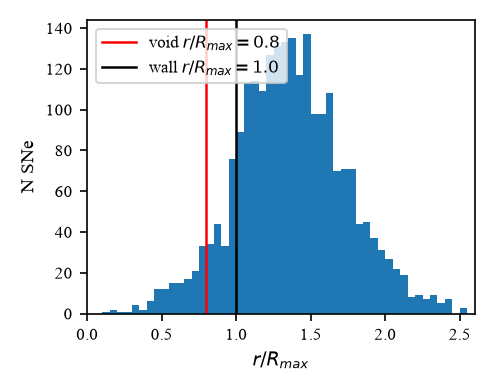
\includegraphics[width=\columnwidth]{../plots/rRv_hist_v2.png}
\caption{$r/R_{\max}$ distribution with 0.8 (void) and 1.0 (wall) lines.}
\label{fig:rrv}
\end{figure}
\begin{figure}
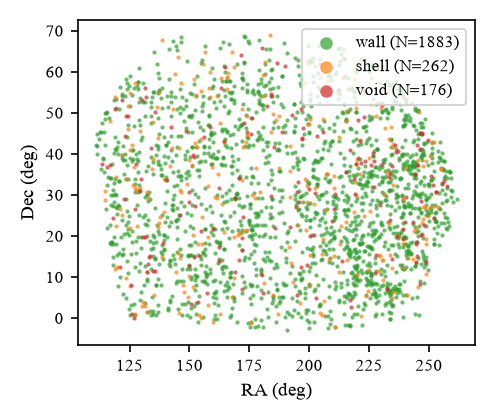
\includegraphics[width=\columnwidth]{../plots/footprint_v2.png}
\caption{Masked RA--Dec distribution colour-coded by environment.}
\label{fig:foot}
\end{figure}
FRB error budget (Cat1): per-sightline $\sigma_{\rm tot}\sim150$--$200\,{\rm pc\,cm^{-3}}$ (IGM 80--120, host 80--150, Milky Way residual 20--40 with NE2001$-$YMW16 median $-3.3$, std $37.5$, p90 $68.1$, halo 20). Void signal $\sim10$--$30$. A $\delta{\rm DM}<50$ limit at 95 per cent needs $N_{\rm void}\gtrsim36$ ($\sim200$ localised total); unlocalised $z<0.114$ needs $\sim900$ void sightlines, have $\sim30$--$50$.
\section{Systematics and next steps}
Peculiar velocities, selection efficiency, host masses, calibration, threshold grid for Hubble residuals, subtype cleaning done for counts, nulls (RA-shuffle within footprint, block bootstrap, 0.00/0.05 mag injection) planned. No unblinding until budget closed.
\section{Data availability}
VAST Zenodo DOI, BTS query URL and date with CSV hash, CHIME Vizier DOI, derived \path{b3_match_v2.parquet} with scripts tag v0.2 on GitHub on acceptance (reviewer token on request).
\clearpage
\begin{thebibliography}{99}
\bibitem[Douglass et al.(2023)]{douglass23} Douglass K.~A.\ et al., 2023, ApJS, 265, 7
\bibitem[Perley et al.(2020)]{perley20} Perley D.~A.\ et al., 2020, ApJ, 904, 35
\bibitem[Fremling et al.(2019)]{fremling19} Fremling C.\ et al., 2019, arXiv:1910.12973
\bibitem[CHIME(2021)]{chime21} CHIME/FRB Collab., 2021, ApJS, 257, 59
\bibitem[CHIME(2026)]{chime26} CHIME/FRB Collab., 2026, arXiv:2601.09399
\bibitem[Wang et al.(2026)]{wang26} Wang et al., 2026, ApJ, 997, 121
\bibitem[Sharma et al.(2026)]{sharma26} Sharma et al., 2026, arXiv:2605.01994
\bibitem[Tsaprazi et al.(2021)]{tsaprazi21} Tsaprazi et al., 2021, MNRAS
\bibitem[Aubert et al.(2025)]{aubert25} Aubert et al., 2025, A\&A, 694, A7
\bibitem[Walker et al.(2024)]{walker24} Walker et al., 2024, A\&A, 683, A71
\bibitem[Macquart et al.(2020)]{macquart20} Macquart et al., 2020, Nature, 581, 391
\end{thebibliography}
\end{document}
